\documentclass{article}

\usepackage{hyperref}
\hypersetup{pdfauthor={Cristian Adrián Ontivero}}
\usepackage[utf8]{inputenc}
\usepackage{graphicx}
\usepackage{gensymb} % for the degree symbol
\usepackage{caption}
\usepackage{float}
\usepackage{color}
\usepackage{mathtools}
\usepackage[hang,flushmargin]{footmisc} 

% For the commutative diagrams.
\usepackage{tikz-cd}

\usepackage{tikz}
\usetikzlibrary{automata, positioning, arrows,
shapes,
fit, % for the dashed boxes on Thompson's construction
calc
}
\tikzset{%
  node distance=3cm, % specifies the minimum distance between two nodes. Change if necessary.
  every state/.style={thick}, % sets the properties for each ’state’ node
  double distance=2.5pt,
  shorten >= 2pt, shorten <= 2pt,
  initial text=$ $,
  every edge/.style={%
    draw,->, >=stealth, auto, semithick
  }
}
\graphicspath{{imgs/}}

\definecolor{darkblue}{RGB}{49,130,189}

\newlength\tindent
\setlength{\tindent}{\parindent}
\setlength{\parindent}{0pt}
\renewcommand{\indent}{\hspace*{\tindent}}

%These tell TeX which packages to use.
\usepackage{array,epsfig}
\usepackage{amsmath}
\usepackage{amsfonts}
\usepackage{amssymb}
\usepackage{amsxtra}
\usepackage{amsthm}
\usepackage{mathrsfs}

%Here I define some theorem styles and shortcut commands for symbols I use often
\theoremstyle{definition}

\newcommand{\lra}{\longrightarrow}
\newcommand{\ra}{\rightarrow}
\newcommand{\surj}{\twoheadrightarrow}
\newcommand{\graph}{\mathrm{graph}}
\newcommand{\bb}[1]{\mathbb{#1}}
\newcommand{\Z}{\bb{Z}}
\newcommand{\Q}{\bb{Q}}
\newcommand{\R}{\bb{R}}
\newcommand{\C}{\bb{C}}
\newcommand{\N}{\bb{N}}
\newcommand{\M}{\mathbf{M}}
\newcommand{\m}{\mathbf{m}}
\newcommand{\MM}{\mathscr{M}}
\newcommand{\HH}{\mathscr{H}}
\newcommand{\Om}{\Omega}
\newcommand{\Ho}{\in\HH(\Om)}
\newcommand{\bd}{\partial}
\newcommand{\del}{\partial}
\newcommand{\bardel}{\overline\partial}
\newcommand{\textdf}[1]{\textbf{\textsf{#1}}\index{#1}}
\newcommand{\ip}[2]{\left\langle{#1},{#2}\right\rangle}
\newcommand{\inter}[1]{\mathrm{int}{#1}}
\newcommand{\exter}[1]{\mathrm{ext}{#1}}
\newcommand{\cl}[1]{\mathrm{cl}{#1}}
\newcommand{\ds}{\displaystyle}
\newcommand{\vol}{\mathrm{vol}}
\newcommand{\cnt}{\mathrm{ct}}
\newcommand{\osc}{\mathrm{osc}}
\newcommand{\LL}{\mathbf{L}}
\newcommand{\UU}{\mathbf{U}}
\newcommand{\support}{\mathrm{support}}
\newcommand{\AND}{\;\wedge\;}
\newcommand{\OR}{\;\vee\;}
\newcommand{\Oset}{\varnothing}
\newcommand{\st}{\ni}
\newcommand{\wh}{\widehat}

\newcommand{\PS}{\mathcal{P}}
\newcommand{\set}[1]{\left\{#1\right\}}
\newcommand{\bra}[1]{\left[#1\right]}
\newcommand{\abs}[1]{\left|#1\right|}
\newcommand{\ec}[1]{{\left[#1\right]}_{\sim}}
\newcommand{\id}{\mathrm{id}}
\newcommand{\cod}{\mathrm{cod~}}
\newcommand{\dom}{\mathrm{dom~}}
\newcommand{\im}{\mathrm{im~}}
\newcommand{\thra}{\twoheadrightarrow}
\newcommand{\emptystr}{\varepsilon}
\newcommand{\emptylan}{\emptyset}
\newcommand{\pdv}[2]{\partial_{#1} \bigl(#2\bigr)}

%Pagination stuff.
\setlength{\topmargin}{-.3 in}
\setlength{\oddsidemargin}{0in}
\setlength{\evensidemargin}{0in}
\setlength{\textheight}{9.in}
\setlength{\textwidth}{6.5in}
\pagestyle{empty}

% The problem environment is a regular ams theorem environment with "Problem"
% text and some leading space to give some separation between the problems.
\theoremstyle{definition}
\newtheorem{problem-internal}{Problem}[subsection]
\newenvironment{problem}{
  \medskip
  \begin{problem-internal}
}{
  \end{problem-internal}
}

% The solution environment is a proof environment with the "solution" text as
% well as the following adjustments:
% - No indent on paragraphs;
% - A small amount of space between paragraphs.
%
% Note: The negative space at the beginning is to remove the space before the
% first paragraph in the solution.
%\newenvironment{solution}{%
  %\begin{proof}[Solution]
  %\vspace{-8px}
  %\setlength{\parskip}{4px}
  %\setlength{\parindent}{0px}
%}{
  %\end{proof}
%}
\theoremstyle{definition}
\newtheorem{solution-internal}{}[subsection]
\newenvironment{solution}{
  \begin{solution-internal}
}{
  \end{solution-internal}
}

% The chngcntr ("change counter") package is used here so that subsection
% numbers are written without the leading section number. This takes place in
% the subsection headings as well as the theorem environment numbering.
%
% Before:
% 1. Section
% 1.1. Subsection
% Problem 1.1.1. What is 1 + 1?
% Problem 1.1.2. What is 1 + 2?
%
% After:
% 1. Section
% 1. Subsection
% Problem 1.1. What is 1 + 1?
% Problem 1.2. What is 1 + 2?
\usepackage{chngcntr}
\counterwithout{subsection}{section}

% Renewing the \thesection command changes the section numbers to roman
% numerals. This matches the style of the Aluffi textbook.
%
% Before:
% 1. Section
% 1.1. Subsection
%
% After:
% I. Section
% I.1. Subsection
%\renewcommand{\thesection}{\Roman{section}} 
%\renewcommand{\thesubsection}{\Roman{subsection}} 

\begin{document}

\section*{Session 1}
\setcounter{section}{1}
\setcounter{subsection}{1}

\begin{solution}
Any ``product type'' (a la Haskell).
Combine two points in a line to get a point in a plane:
\begin{center}
\begin{tikzcd}
(x,y) \arrow[r] \arrow[d] & y \\
x
\end{tikzcd}
\end{center}

Morning activities: sleep, clean, read.
Afternoon activities: go for a walk, go to a coffee shop, take a nap.
\begin{center}
\begin{tikzcd}
\text{Day Activities} \arrow[r] \arrow[d] & \text{Afternoon Activities} \\
\text{Morning Activities}
\end{tikzcd}
\end{center}
etc.

\end{solution}

% Session 1, ex. 2
\begin{solution}
TODO 
\end{solution}

\section*{Article I}
\renewcommand{\thesection}{\Roman{section}} 
\renewcommand{\thesubsection}{\Roman{subsection}} 
\setcounter{solution-internal}{0}

% Page 18, exercise 1
\begin{solution}
The maps would be as follows:

\begin{tikzpicture}[node distance=16pt, every node/.style={shape=circle, inner sep=1pt, minimum size=2pt}, >=latex]

\node[fill=black] (a0) {};
\node[fill=black, below=of a0] (a1) {};
\node[fill=black, below=of a1] (a2) {};
\node[draw, shape=ellipse,minimum size=1cm,fit={(a0) (a2)}] (e0) {};
\node[above=2pt of e0] (l0) {A};

\node[fill=black, right=4cm of a0] (b0) {};
\node[fill=black, below left=0.7cm and 0.2cm of b0] (b1) {};
\node[fill=black, below right=0.2cm and 0.4cm of b1] (b2) {};
\node[fill=black, right=4cm of a2] (b3) {};
\node[draw, shape=ellipse,minimum size=1cm,fit={(b0) (b3)}] (e1) {};
\node[above=2pt of e1] (l1) {B};

\node[fill=black, right=8cm of a0] (d0) {};
\node[fill=black, right=8cm of a1] (d1) {};
\node[fill=black, right=8cm of a2] (d2) {};
\node[fill=black, right=8pt of d0] (d3) {};
\node[fill=black, right=8pt of d1] (d4) {};
\node[fill=black, right=8pt of d2] (d5) {};
\node[draw, shape=ellipse,minimum size=1.3cm,fit={(d0) (d5)}] (e2) {};
\node[above=2pt of e2] (l2) {D};

%\node[below=1.5cm of aux2,font=\Large\bfseries] {Range};

\draw[->] (a0) edge[out=5, in=175] node {$f$} (b0);
\draw[->] (a1) edge[out=10, in=170] (b1);
\draw[->] (a2) edge[out=10, in=180] (b2);

\draw[->] (b0) edge[out=5, in=175] node {$h \circ g$} (d0);
\draw[->] (b1) edge[out=10, in=200] (d0);
\draw[->] (b2) edge[out=10, in=180] (d1);
\draw[->] (b3) edge[out=10, in=180] (d2);

\node[fill=black, below=2cm of a2] (aa0) {};
\node[fill=black, below=of aa0] (aa1) {};
\node[fill=black, below=of aa1] (aa2) {};
\node[draw, shape=ellipse,minimum size=1cm,fit={(aa0) (aa2)}] (e3) {};
\node[above=2pt of e3] (ll0) {A};

\node[fill=black, right=8cm of aa0] (dd0) {};
\node[fill=black, right=8cm of aa1] (dd1) {};
\node[fill=black, right=8cm of aa2] (dd2) {};
\node[fill=black, right=8pt of dd0] (dd3) {};
\node[fill=black, right=8pt of dd1] (dd4) {};
\node[fill=black, right=8pt of dd2] (dd5) {};
\node[draw, shape=ellipse,minimum size=1.3cm,fit={(dd0) (dd5)}] (e4) {};
\node[above=2pt of e4] (ll1) {D};

\draw[->] (aa0) edge[out=5, in=175] node[yshift=-0.5cm] {$(h \circ g) \circ f$} (dd0);
\draw[->] (aa1) edge[out=5, in=185] (dd0);
\draw[->] (aa2) edge[out=10, in=190] (dd1);

\end{tikzpicture}
\end{solution}

\begin{solution}
$2\cdot 2\cdot 2 = 2^4$
\end{solution}

\begin{solution}
$3^3 = 27$
\end{solution}

\begin{solution}
$3^2 = 9$
\end{solution}
\begin{solution}
$2^4 = 16$ 
\end{solution}

The previous four exercises are instances of the more general $\abs{\cod f}^{\abs{\dom f}}$.

\begin{solution}
If $f(x) = y$, we need that $f(y) = y$. Thus, the answer is 10 maps. Graphically:
\begin{center}
\begin{tikzpicture}[node distance=4pt, every node/.style={fill=black, shape=circle, inner sep=1pt, minimum size=2pt}, >=latex]

\node (a0) {};
\node[below=of a0] (a1) {};
\node[below=of a1] (a2) {};
\node[right=16pt of a0] (b0) {};
\node[below=of b0] (b1) {};
\node[below=of b1] (b2) {};
\draw (a0) -- (b0);
\draw (a1) -- (b1);
\draw (a2) -- (b2);

\node[right=1cm of b0] (c0) {};
\node[below=of c0] (c1) {};
\node[below=of c1] (c2) {};
\node[right=16pt of c0] (d0) {};
\node[below=of d0] (d1) {};
\node[below=of d1] (d2) {};
\draw (c0) -- (d0);
\draw (c1) -- (d0);
\draw (c2) -- (d0);

\node[right=1cm of d0] (e0) {};
\node[below=of e0] (e1) {};
\node[below=of e1] (e2) {};
\node[right=16pt of e0] (f0) {};
\node[below=of f0] (f1) {};
\node[below=of f1] (f2) {};
\draw (e0) -- (f1);
\draw (e1) -- (f1);
\draw (e2) -- (f1);

\node[right=1cm of f0] (g0) {};
\node[below=of g0] (g1) {};
\node[below=of g1] (g2) {};
\node[right=16pt of g0] (h0) {};
\node[below=of h0] (h1) {};
\node[below=of h1] (h2) {};
\draw (g0) -- (h2);
\draw (g1) -- (h2);
\draw (g2) -- (h2);

\node[right=1cm of h0] (i0) {};
\node[below=of i0] (i1) {};
\node[below=of i1] (i2) {};
\node[right=16pt of i0] (j0) {};
\node[below=of j0] (j1) {};
\node[below=of j1] (j2) {};
\draw (i0) -- (j0);
\draw (i1) -- (j0);
\draw (i2) -- (j2);

\node[below=0.5cm of a2] (aa0) {};
\node[below=of aa0] (aa1) {};
\node[below=of aa1] (aa2) {};
\node[right=16pt of aa0] (bb0) {};
\node[below=of bb0] (bb1) {};
\node[below=of bb1] (bb2) {};
\draw (aa0) -- (bb1);
\draw (aa1) -- (bb1);
\draw (aa2) -- (bb2);

\node[right=1cm of bb0] (cc0) {};
\node[below=of cc0] (cc1) {};
\node[below=of cc1] (cc2) {};
\node[right=16pt of cc0] (dd0) {};
\node[below=of dd0] (dd1) {};
\node[below=of dd1] (dd2) {};
\draw (cc0) -- (dd0);
\draw (cc1) -- (dd1);
\draw (cc2) -- (dd1);

\node[right=1cm of dd0] (ee0) {};
\node[below=of ee0] (ee1) {};
\node[below=of ee1] (ee2) {};
\node[right=16pt of ee0] (ff0) {};
\node[below=of ff0] (ff1) {};
\node[below=of ff1] (ff2) {};
\draw (ee0) -- (ff0);
\draw (ee1) -- (ff2);
\draw (ee2) -- (ff2);

\node[right=1cm of ff0] (gg0) {};
\node[below=of gg0] (gg1) {};
\node[below=of gg1] (gg2) {};
\node[right=16pt of gg0] (hh0) {};
\node[below=of hh0] (hh1) {};
\node[below=of hh1] (hh2) {};
\draw (gg0) -- (hh0);
\draw (gg1) -- (hh1);
\draw (gg2) -- (hh0);

\node[right=1cm of hh0] (ii0) {};
\node[below=of ii0] (ii1) {};
\node[below=of ii1] (ii2) {};
\node[right=16pt of ii0] (jj0) {};
\node[below=of jj0] (jj1) {};
\node[below=of jj1] (jj2) {};
\draw (ii0) -- (jj2);
\draw (ii1) -- (jj1);
\draw (ii2) -- (jj2);

\end{tikzpicture}
\end{center}
\end{solution}

% Exercise 7
\begin{solution}
Three.

\begin{center}
\begin{tikzpicture}[node distance=4pt, every node/.style={fill=black, shape=circle, inner sep=1pt, minimum size=2pt}, >=latex]

\node (a0) {};
\node[below=of a0] (a1) {};
\node[right=16pt of a0] (b0) {};
\node[below=of b0] (b1) {};
\draw (a0) -- (b0);
\draw (a1) -- (b1);

\node[right=1cm of b0] (c0) {};
\node[below=of c0] (c1) {};
\node[right=16pt of c0] (d0) {};
\node[below=of d0] (d1) {};
\draw (c0) -- (d1);
\draw (c1) -- (d1);

\node[right=1cm of d0] (e0) {};
\node[below=of e0] (e1) {};
\node[right=16pt of e0] (f0) {};
\node[below=of f0] (f1) {};
\draw (e0) -- (f0);
\draw (e1) -- (f0);
\end{tikzpicture}
\end{center}
\end{solution}


\begin{solution}
In other words, how many invertible functions (iso arrows) are there? It's not possible, because $\abs{B} < \abs{A}$. Thus you ``lose information'' and the
transformation can't be reversed.
\end{solution}

\begin{solution}

Yes, because $\abs{A} > \abs{B}$ (it needs to be at least equal). There are
$3\cdot 2 = 6$ possible invertible functions for $h$. As for $k$, since there is
an element we don't care about, which can be mapped to whatever element in B,
there are $6 \cdot 2 = 12$ possibilities. Thus, there are $6 \cdot 12 = 72$ possible pairs.

\end{solution}

\section*{Session 3}
\setcounter{subsection}{3}
\renewcommand{\thesection}{\arabic{section}} 
\renewcommand{\thesubsection}{\arabic{subsection}}
\setcounter{solution-internal}{0}

\begin{solution}
(a) makes sense, $k\circ h \circ g \circ f \colon A \to B$. (c) also: $g\circ f \circ g \circ k \circ h \colon A \to A$
\end{solution}

% There isn't much to Ex.2 

\section*{Article II}
\setcounter{subsection}{2}
\renewcommand{\thesubsection}{\Roman{subsection}}
\setcounter{solution-internal}{0}

\begin{solution}
$ $ %needed for the list to align properly
\begin{itemize}
\item Reflexive: $1_A$ is its own inverse: $1_A \circ 1_A = 1_A$.
\item Symmetric: $g^{-1} = f$, since $g \circ f = 1_A$ and $f \circ g = 1_B$.
\item Transitive: ${(k \circ f)}^{-1} = f^{-1} \circ k^{-1}$. Note that we know
that $f^{-1}$ and $k^{-1}$ exist, since $f$ and $k$ are iso. Then: 

\begin{minipage}{.4\textwidth}
\begin{align*}
  (k \circ f) \circ {(k \circ f)}^{-1} &= (k \circ f) \circ k^{-1} \circ f^{-1} \\
   &= k \circ (f \circ f^{-1}) \circ k^{-1} \\
   &= k \circ 1_B \circ k^{-1} \\
   &= k \circ k^{-1} \\
   &= 1_C
\end{align*}
\end{minipage}\hspace{32pt}%
\begin{minipage}{.4\textwidth}
\begin{align*}
  {(k \circ f)}^{-1} \circ (k \circ f) &=  f^{-1} \circ k^{-1} \circ (k \circ f) \\
   &= f^{-1} \circ (k^{-1} \circ k) \circ f \\
   &= f^{-1} \circ 1_B \circ f \\
   &= f^{-1} \circ f \\
   &= 1_A
\end{align*}
\end{minipage}
\end{itemize}
\end{solution}

\begin{solution}
\[
\arraycolsep=2pt
\begin{array}{rcl}
  1_B                      & = & 1_B \\
  f \circ g                & = & f \circ k \\
  f^{-1} \circ (f \circ g) & = & f^{-1} \circ (f \circ k) \\
  (f^{-1} \circ f) \circ g & = & (f^{-1} \circ f) \circ k \\
  1_A \circ g              & = & 1_A \circ k \\
  g                        & = & k
\end{array}
\]
\end{solution}

\begin{solution}
$ $%
\begin{itemize}
\item[(a)]
\[
\arraycolsep=2pt
\begin{array}{rcl}
  f \circ h              & = & f \circ k \\
  f^{-1} \circ f \circ h & = & f^{-1} \circ f \circ k \\
  1_A \circ h            & = & 1_A \circ k \\
  h                      & = & k
\end{array}
\]
\item[(b)]
\[
\arraycolsep=2pt
\begin{array}{rcl}
  h \circ f              & = & k \circ f \\
  h \circ f \circ f^{-1} & = & k \circ f \circ f^{-1} \\
  h \circ 1_B            & = & k \circ 1_B \\
  h                      & = & k
\end{array}
\]
\end{itemize}

\end{solution}
\begin{solution}
$ $
\begin{enumerate} 
\item $f^{-1}(x) = \frac{x-7}{3}$
\item $g^{-1}(x) = \sqrt{x}$
\item Doesn't have, since $g\colon \R \to \R$ isn't monic, e.g.: $2^2 = {(-2)}^2$, but $2 \neq -2$
\item Same problem as before, although now $g$ is epic.
\item $y = \frac{1}{x+1} \Rightarrow \frac{1}{y} = x + 1 \Rightarrow \frac{1}{y} - 1 = x$

$\ell^{-1}(x) = \frac{1}{x} - 1$, but $\ell^{-1}(0)$ is undefined.
Thus it is not invertible. $l(x)$ itself isn't epic, for instance $\nexists x (l(x) = 0)$.
\end{enumerate} 
\end{solution}

\begin{solution}
$f(0)$ can be $b$, $p$ or $q$, and $f(1)$ can be $r$ or $s$. Thus $3 \cdot 2 = 6$
\end{solution}

\begin{solution}
$t = g \circ r$.

\begin{center}
\begin{tikzcd}
& B \arrow[rd, dashed, "t?"] \arrow[ld, "r", out=240, in=20] & \\
A \arrow [ru, "f"] \arrow[rr, "g"'] & & T 
\end{tikzcd}
\end{center}

We see that it satisfies the required equation: $t \circ f = g \circ r \circ f = g \circ 1_A = g$.
\end{solution}

\begin{solution}
$ $\newline
\begin{minipage}{.4\textwidth}
\[ 
\arraycolsep=2pt
\begin{array}{rcl}
  t_1 \circ f &=& t_2 \circ f \\
  (t_1 \circ f) \circ s &=& (t_2 \circ f) \circ s \\
  t_1 \circ (f \circ s) &=& t_2 \circ (f \circ s) \\
  t_1 \circ 1_B &=& t_2 \circ 1_B \\
  t_1 &=& t_2 \\
\end{array}
\]
\end{minipage}%
\begin{minipage}{.4\textwidth}
\begin{tikzcd}
B \ar[r, "s"] \ar[rr, "1_B"', bend right] & A \arrow[r, "f"] & B \ar[r, shift left, "t_1"] \ar[r, shift right, "t_2"'] & T \\
\end{tikzcd}
\end{minipage}%
\end{solution}

% Exercise 8
\begin{solution}
Given $f\colon A \to B$ with section $s\colon B \to A$, and $g\colon B \to C$ with section $s'\colon C \to D$, we take $s'' = s \circ s'$. Then:
\[ (g \circ f) \circ s'' = g \circ f \circ (s \circ s') = g \circ (f \circ s) \circ s' = g \circ 1_B \circ s' = g \circ s' = 1_C \]

Therfore $s''$ is a section for $g \circ f$.
\end{solution}

% Exercise 9
\begin{solution}
Suppose $r$ is a retraction for $f$ (i.e. $r \circ f = 1_A$), and let $e = f \circ r$. Then:
\[ e \circ e = (f \circ r) \circ (f \circ r) = f \circ (r \circ f) \circ r = f \circ 1_A \circ r = f \circ r = e \]
If $f$ is an isomorphism, then $r$ is its inverse, by the uniqueness of
inverses theorem (this is introduced just after the exercise; another
justification would be exercise 2). Thus $e = f \circ r = 1_B$.
\end{solution}

% Exercise 10
% Same as 3.4.3 from Topoi: The Categorial Analysis of Logic
\begin{solution}
TODO
\end{solution}

% Exercise 11
\begin{solution}
An example of an isomorphism $A \xrightarrow{\mathmakebox[12pt]{f}} B$ is given by:

\begin{center}
\begin{tikzpicture}[node distance=1pt, every node/.style={minimum height=10pt,  minimum width=28pt}, >=latex]

\node[font=\footnotesize] (a0) {Fatima};
\node[below=0pt of a0, font=\footnotesize] (a1) {Omer};
\node[below=0pt of a1, font=\footnotesize] (a2) {Alysia};
\node[shape=ellipse, draw, fit={(a0) (a2)}] (e0) {};
\node[above=0pt of e0] (l0) {A};

\node[right=2cm of a0, font=\footnotesize] (b0) {Coffee};
\node[below=0pt of b0, font=\footnotesize] (b1) {Tea};
\node[below=0pt of b1, font=\footnotesize] (b2) {Cocoa};
\node[shape=ellipse, draw, minimum size=1cm,fit={(b0) (b2)}] (e1) {};
\node[above=0pt of e1] (l1) {B};

\node[right=2cm of b0, font=\footnotesize] (c0) {Fatima};
\node[below=0pt of c0, font=\footnotesize] (c1) {Omer};
\node[below=0pt of c1, font=\footnotesize] (c2) {Alysia};
\node[shape=ellipse, draw, fit={(c0) (c2)}] (e2) {};
\node[above=0pt of e2] (l2) {A};

\draw[->] (a0) edge[out=5, in=175] node {$f$} (b0);
\draw[->] (a1) edge[out=5, in=175] (b1);
\draw[->] (a2) edge[out=5, in=175] (b2);
\draw[->] (b0) edge[out=5, in=175] node {$f^{-1}$} (c0);
\draw[->] (b1) edge[out=5, in=175] (c1);
\draw[->] (b2) edge[out=5, in=175] (c2);

\end{tikzpicture}
\end{center}
It is not possible to find an isomorphism $A \to C$ because $\abs{A} > \abs{C}$.
\end{solution}
\begin{solution}
The are $3!$ isomorphisms. As for endomaps of $A$, there are also $3!$, namely:
\begin{center}
\begin{tikzpicture}[node distance=4pt, every node/.style={fill=black, shape=circle, inner sep=1pt, minimum size=2pt}, >=latex]

\node (a0) {};
\node[below=of a0] (a1) {};
\node[below=of a1] (a2) {};
\node[right=16pt of a0] (b0) {};
\node[below=of b0] (b1) {};
\node[below=of b1] (b2) {};
\draw (a0) -- (b0);
\draw (a1) -- (b1);
\draw (a2) -- (b2);

\node[right=1cm of b0] (c0) {};
\node[below=of c0] (c1) {};
\node[below=of c1] (c2) {};
\node[right=16pt of c0] (d0) {};
\node[below=of d0] (d1) {};
\node[below=of d1] (d2) {};
\draw (c0) -- (d0);
\draw (c1) -- (d2);
\draw (c2) -- (d1);

\node[right=1cm of d0] (e0) {};
\node[below=of e0] (e1) {};
\node[below=of e1] (e2) {};
\node[right=16pt of e0] (f0) {};
\node[below=of f0] (f1) {};
\node[below=of f1] (f2) {};
\draw (e0) -- (f1);
\draw (e1) -- (f0);
\draw (e2) -- (f2);

\node[right=1cm of f0] (g0) {};
\node[below=of g0] (g1) {};
\node[below=of g1] (g2) {};
\node[right=16pt of g0] (h0) {};
\node[below=of h0] (h1) {};
\node[below=of h1] (h2) {};
\draw (g0) -- (h2);
\draw (g1) -- (h1);
\draw (g2) -- (h0);

\node[right=1cm of h0] (i0) {};
\node[below=of i0] (i1) {};
\node[below=of i1] (i2) {};
\node[right=16pt of i0] (j0) {};
\node[below=of j0] (j1) {};
\node[below=of j1] (j2) {};
\draw (i0) -- (j1);
\draw (i1) -- (j2);
\draw (i2) -- (j0);

\node[right=1cm of j0] (x0) {};
\node[below=of x0] (x1) {};
\node[below=of x1] (x2) {};
\node[right=16pt of x0] (z0) {};
\node[below=of z0] (z1) {};
\node[below=of z1] (z2) {};
\draw (x0) -- (z2);
\draw (x1) -- (z0);
\draw (x2) -- (z1);

\end{tikzpicture}
\end{center}
$27$ would be $3^3$, the number of distinct maps from $A$ to $A$ (or $A$ to $B$).
\end{solution}

\section*{Session 4}
\setcounter{subsection}{4}
\renewcommand{\thesection}{\arabic{section}} 
\renewcommand{\thesubsection}{\arabic{subsection}}
\setcounter{solution-internal}{0}

\begin{solution}
We check that $h \circ d$ and $d \circ h$ are identity maps.
\[
\arraycolsep=2pt\renewcommand{\arraystretch}{1.3}
\begin{array}{rl p{1cm} rl}
  (h \circ d)(x) &= h (d (x)) & &    (d \circ h)(x) &= d (h (x)) \\
                 &= h (2 x) & &                   &= d (\frac{1}{2} x) \\
                 &= \frac{1}{2} (2 x) & &         &= 2 (\frac{1}{2} x) \\
                 &= (\frac{1}{2} \cdot 2) x & &   &= (2 \cdot \frac{1}{2}) x\\
                 &= x & &                           &= x
\end{array}
\]
\end{solution}
\begin{solution}
\newcommand{\od}{\mathrm{odd}}
\newcommand{\ev}{\mathrm{even}}
\newcommand{\np}{\mathrm{negative}}
\newcommand{\po}{\mathrm{positive}}

We take $f$ such that $f(\od) = \np$, and $f(\ev) = \po$.
Then:
\begin{align*}
f(\od + \od) & = f(\od) \times f(\od) = \np \times \np = \po \\
f(\od + \ev) & = f(\od) \times f(\ev) = \np \times \po = \np \\
f(\ev + \ev) & = f(\ev) \times f(\ev) = \po \times \po = \po \\
f^{-1}(\np \times \np) & = f^{-1}(\np) + f^{-1}(\np) = \od + \od = \ev \\
f^{-1}(\po \times \np) & = f^{-1}(\po) + f^{-1}(\np) = \ev + \od = \od \\
f^{-1}(\po \times \po) & = f^{-1}(\po) + f^{-1}(\po) = \ev + \ev = \ev \\
\end{align*}
The other invertible map doesn't respect the combining rules.
\end{solution}

\end{document}
